\section{An Overview of BIP32-based HD Wallets}
\label{sec:bip32}

Hierarchical Deterministic Wallets (HD wallets, for short) in the cryptocurrency
domain derive from the BIP32 specification%
\footnote{\url{https://github.com/bitcoin/bips/blob/master/bip-0032.mediawiki}.
  Last access, December 13th, 2021.}
The motivation behind creating this type of wallets is clear if one thinks about
how typical cryptocurrency systems work: each address is associated with a key
pair and, in order to achieve high security and privacy levels, it is best to
limit the reusage of addresses (thus, key pairs). Therefore, a too high number
of needed key pairs is quickly reached. If each key is generated independently
at random, management becomes too complex -- especially, if several devices
are expected to be synchronised. As a solution to this challenge, a hierachical
tree-based data structure was proposed, in which each parent node can be used to
derive multiple child nodes, deterministically. This approach seems also useful
to foster some sort of separation -- i.e., create sub-trees that are
(computationally) independent from one another, in the sense that a compromise
in one does not lead to a compromise in the other. Typically, the root node
of the tree is derived from a seed encoded as a mnemonic. BIP39%
\footnote{\url{https://github.com/bitcoin/bips/blob/master/bip-0039.mediawiki}.
  Last access, December 13th, 2021.} is the main specification for this purpose.

In this section, we give a brief overview of the BIP32 specification, and
provide a ``full path'' from mnemonic to key pair. To avoid repeating already
well documented processes, the overview will refer to the specifications when
appropriate.
%
In a final subsection, we will also overview how does all this apply to the
Cardano Lightwallet and Atala Prism cases.

\subsection{Main Specifications}

While the main specification is BIP32, it essentially gives the main guidelines
to create HD wallets. To avoid ambiguity leading to incompatible
implementations, BIP43%
\footnote{\url{https://github.com/bitcoin/bips/blob/master/bip-0043.mediawiki}.
  Last access, December 13th, 2021.} and BIP44%
\footnote{\url{https://github.com/bitcoin/bips/blob/master/bip-0044.mediawiki}.
  Last access, December 13th, 2021.} specify how to organize HD wallets so
that the resulting tree structure enables the most common use cases (which, at
least initially, focus on the cryptocurrency scenario). In addition, the
specification that defines how to encode (pseudo-)random bitstrings as
mnemonic is given in BIP39.

\subsection{Main Concepts}

\begin{description}
\item[HD wallet tree structure.] HD wallets are organised as trees, where the
  root node is directly derived from the main seed (typically, a mnemonic-encoded
  random string). We denote the root level with level $0$, and all descendants
  with increasing numbers. A level other than the root level can have an
  arbitrary number of nodes.
\item[(Child) Index.] The child index just identifies how many childs can be (or
  have been) created before the current child, at the current depth of the tree.
  We assume $0$ to be the first index.
\item[Chaincode.] To introduce extra ``non-determinism'' in the way child keys
  are derived from parent keys, part of the pseudo-randomly derived data is
  used as key for pseudo-random derivations of lower levels. This part of the
  derived data is referred to as chaincode. We will denote the chaincode of the
  $j$-th node at level $i$ of the tree with $c_{i,j}$.
\item[Extended keys.] An extended public (resp. private) key is composed by the
  public (resp. private) key and the chaincode.  
\item[Hardened child keys.] A hardened child key can only be derived from the
  parent private key, and the parent key chaincode. 
\item[Non-hardened child keys.] A non-hardened child key can be derived both
  from the parent private and parent public key, and the parent key chaincode.
\end{description}

\paragraph{Hardened vs non-hardened child derivation.}

\paragraph{Isolation of HD partitions.} In the following section, we use
the concept of isolated and non-isolated partitions. This is something that is
only indirectly mentioned in the BIPs and other related works, but which is of
crucial importance in order to limit the impact of compromised keys. Namely,
assume that a child key is derived in non-hardened mode. Then, if the extended
parent public key is leaked, as well as the private (non-extended) child key, it
is possible to extract the parent private key -- and, therefore, all the keys
(private and public; hardened or not) that derive from it. If child keys are
derived in hardened mode, this does not apply. For the sake of clarity, we
illustrate the difference through the diagram in \figref{fig:isolation}.

\begin{figure}[ht!]
  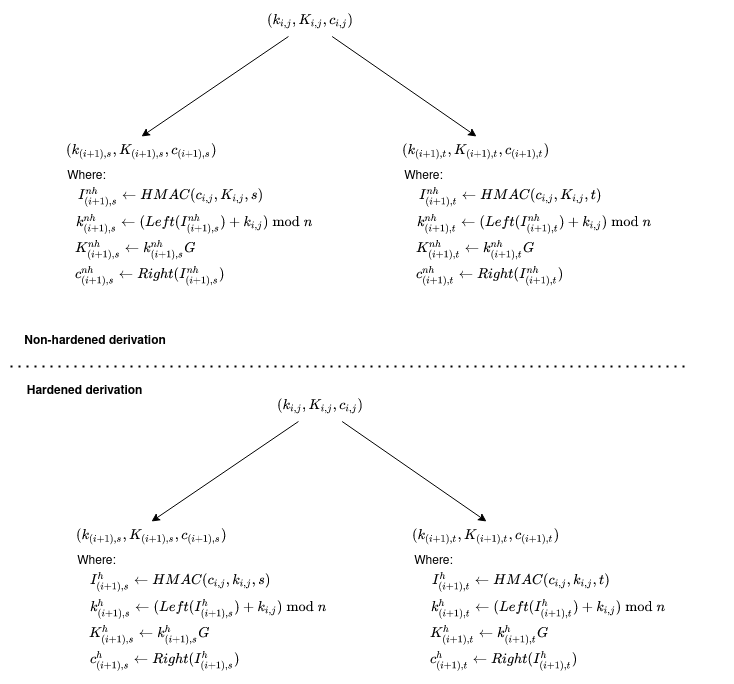
\includegraphics[width=\textwidth]{figures/child_derivation.png}
  \caption{Partition isolation through hardened child derivation. $G$ is the
    base point of the underlying elliptic curve, and $n$ is the order of
    the associated group.}
  \label{fig:isolation}
\end{figure}

Assume that the extended public key $(K_{i,j}, c_{i,j})$ is compromised, along
with its child private non-hardened key $k^{nh}_{(i+1),t}$. Then, it is
straightforward  to recompute the \emph{parent} private key $k_{i,j}$
(indedpendently on whether it was derived in hardened mode or not) as:
$k_{i,j} \leftarrow (K_{(i+1),t}^{nh} - Left(I_{(i+1),t}^{nh})) \bmod n$.
Obviously, given the parent private key $k_{i,j}$, it is straightforward to
derive all its descendants (hardened or not), as well as recursively apply the
same strategy, should any ancestor be also compromised.

\subsection{From Mnemonic to Key Pairs: High-level Overview}

The following description is based on BIP39 for the processing of mnemonics,
and BIP44 (which is a restriction to BIP43 and BIP32) for the structure of
an HD wallet.

\paragraph{From (pseudo-)random bitstrings to mnemonics, and back.}

\paragraph{Layer 1: \emph{isolated} partitions per \texttt{purpose}}

\paragraph{Layer 2: \emph{isolated} partitions per \texttt{coin type}}

\paragraph{Layer 3: \emph{isolated} partitions per \texttt{account}}

\paragraph{Layer 4: \emph{non-isolated} partitions per \texttt{visibility}}

\paragraph{Layer 5: Final key pairs}

\subsection{Comments on a Recent Security Evaluation}

\cite{def+21}

%%% Local Variables:
%%% mode: latex
%%% TeX-master: "single-mnemonic"
%%% End:
